\documentclass[jou,apacite]{apa6}
\usepackage{amsmath}
\usepackage{color}
\usepackage{relsize}
\usepackage{float}
\usepackage{graphicx}
\usepackage{mathrsfs}

\title{Does Criterial Learning Depend on Procedural Mechanisms?}
\shorttitle{Is Criterion Learning Procedural}

\author{Psych 10 / 101}
\affiliation{UC Berkeley Psych 10 / 101 Summer Course 2018}

\keywords{associative learning, categorization}
\authornote{Corresponding Author: Matthew Crossley (matthewjohncrossley@gmail.com)}

\abstract{Learning a response criterion is a critical requirement in many
categorization and decision-making tasks. Despite its importance, little is
known about the cognitive and neural processes that mediate criterial learning.
One possibility is that criterial learning relies exclusively on executive
attention and declarative memory-based mechanisms, and another is that criterial
learning is a form of simple associative learning that depends on procedural
memory. Much evidence suggests that short feedback delays interfere with
procedural learning, but not with learning that depends on explicit,
declarative-memory systems. An experiment is described in which we investigated
whether or not short feedback delays impaired criterial learning, relative to
conditions where the feedback immediately followed the response.}

\rightheader{Draft}
\leftheader{Draft}

\begin{document}
\maketitle 

\section{Introduction}
A huge literature suggests that the learning of one-dimensional categorization
rules is primarily an explicit process that depends on a large neural network
that includes the prefrontal cortex (PFC) \cite{AshbyCOVIS1998, BungeWallis2007,
erickson1998rules}. Several different cognitive processes are thought to
underlie rule learning of this nature. For example, the COVIS theory of category
learning \cite{AshbyCOVIS1998} hypothesizes that rule learning includes
subprocesses that select or construct an appropriate rule, maintain the selected
rule in working memory, switch attention from a discredited rule to a new
candidate rule, and learn the appropriate criterion on the relevant stimulus
dimension that separates the two category responses. This latter
criterial-learning process is thought to be ubiquitous in many different
decision-making tasks. For example, it is the only form of learning assumed by
signal detection theory \cite{MacmillanCreelman2005}.

Despite the prevalence of criterial learning, and its key role in explicit tasks
such as rule-based category learning, very little is known about its mediating
cognitive and neural processes. An obvious hypothesis might be that criterial
learning depends on explicit processes, such as executive attention and working
memory. However, unlike the all-or-none nature of other rule-learning processes
such as rule selection, criterial learning seems incremental, in the same way as
category-learning tasks thought to depend on implicit, procedural-learning
systems \cite{SmithEll2015}.

Thus, there are at least two qualitatively distinct possibilities. One is that
criterial learning relies exclusively on PFC-based mechanisms associated with
working memory and executive attention. For example, the criterion might be
learned by holding a representation of a stimulus that has the criterion value
on the relevant dimension in working memory and comparing new stimuli to this
remembered referent. A quite different possibility is that criterial learning is
a form of procedural learning. For example, the criterion might be learned by
initial guessing followed by the gradual formation of stimulus-response
associations.

This article describes the first known direct test of whether criterial learning
is mediated by implicit, procedural-learning processes, or by explicit,
declarative memory-based processes. To test between these two possibilities, we
examined criterial learning when feedback was delayed by several seconds. A
number of studies have reported that short feedback delays interfere with
procedural learning, but even relatively long delays have no effect on learning
that depends on explicit, declarative-memory systems \cite{dunn2012effect,
MaddoxAshbyBohil2003, MaddoxIng2005}.

Much evidence suggests that procedural learning is mediated within the basal
ganglia, and especially at cortical-striatal synapses, where synaptic plasticity
seems to follow reinforcement learning rules \cite{AshbyEnnis2006,
HoukAdamsBarto1995, MishkinEtAl1984, Willingham1998}. Delayed feedback is
thought to impair striatal-mediated procedural learning by interfering with the
basic biochemical processes that mediate cortical-striatal synaptic plasticity.
Synaptic plasticity in the striatum is strongest when the intracellular
signaling cascades driven by NMDA receptor activation and dopamine (DA) D1
receptor activation coincide \cite{LismanSchulmanCline2002, Rudy2014}. The
further apart in time these two cascades peak, the less effect DA will have on
synaptic plasticity. For example, Yagishita et al.
(2014\nocite{YagishitaEtAl2014}) reported that synaptic plasticity was best
[i.e., greatest increase in spine volume on striatal medium spiny neurons
(MSNs)] when DA neurons were stimulated 600 ms after MSNs. When the DA neurons
were stimulated before the MSNs or 5 s after the MSNs, then no evidence of any
plasticity was observed. Similar results have been reported in
information-integration category learning -- which is thought to depend on
procedural learning. First, \citeA{Worthyetal2013} reported that
information-integration learning is best with feedback delays of 500ms and
slightly worse with delays of 0 or 1000ms. Second, several studies have reported
that feedback delays of 2.5 s or longer impair information-integration learning,
whereas delays as long as 10 secs have no effect on the learning of explicit
categorization rules \cite{dunn2012effect, MaddoxAshbyBohil2003, MaddoxIng2005}.

Thus, the critical question addressed in this article is whether criterial
learning is impaired in the presence of feedback delays. 

\section{Materials \& Methods}
\subsection{Participants \& Conditions}
Fifty-nine participants were UCSB undergraduates and received course credit for
their participation. All had normal or corrected to normal vision. We randomly
assigned each participant to one of three conditions (target $N>16$ per
condition based on similar previous research): delayed feedback (Delay: $N =
21$); immediate feedback with a short intertrial interval (ITI) (Short ITI:$ N =
21$); or immediate feedback with a long ITI (Long ITI: $N = 17$). Participants
were excluded from subsequent analyses if they solved fewer than 4 problems over
the course of the entire experiment. This criterion was chosen from inspection
of Figure \ref{hist_nps}, which shows the number of problems solved by each
participant in each condition displayed as histograms. Note that all conditions
-- especially the Short ITI and Long ITI condition -- appear bimodal. The lower
mode corresponds to participants that performed very poorly and were most likely
poorly motivated. The number of participants excluded was not significantly
different among groups [$\chi^2(2) = 0.56, p =.76$], indicating that exclusion
was likely not driven by experiment-specific factors. Forty-five participants
survived this exclusion (Delay: $N = 16$, Short ITI: $N = 17$, Long ITI: $N =
12$).

\subsection{Apparatus}
All experiments were performed in a dimly lit room. Participants sat
approximately 24'' from a 17'' $\times$ 11'' monitor running at a resolution of
1680 $\times$ 1050 pixels. Participants made category judgments by pressing the
`d' or `k' keys on a standard computer keyboard for `A' or `B' choices,
respectively. Stickers with bold print `A' or `B' were placed on the appropriate
keys.

\subsection{Stimuli and Categories}
\begin{figure}
  \centering
  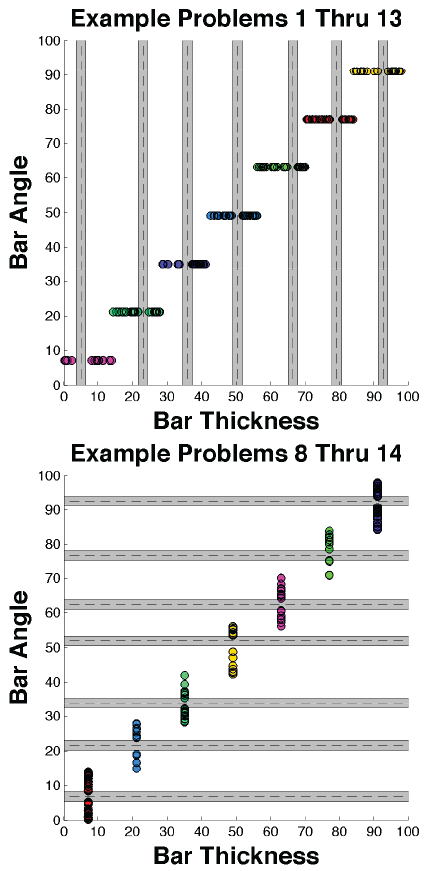
\includegraphics[width=.35\textwidth]{figures/Space.png}
  \caption{Category sample space. Different colors represent different
    category problems. Dashed lines are category boundaries (criterion) and the
    surrounding solid lines mark a no-man's land in which no stimuli were sampled.}
  \label{space}
\end{figure}
Stimuli were circular sine-wave gratings that varied in bar width and bar
orientation, drawn from various 1-dimensional uniform distributions specific to
the current category problem. We first defined an arbitrary 2-dimensional
$[0-100,0-100]$ stimulus space, and then split each dimension of this space into
7 bins of width 14 units each. The structure of the various criterial-learning
tasks is illustrated in Figure \ref{space}. Each criterial-learning problem was
created by first randomly selecting a relevant dimension, and then randomly
selecting one of the 7 bins defined on that dimension. Each bin was also
associated with a corresponding unique value on the irrelevant dimension. We
buffered the to-be-learned response criterion by 10\% of total bin width on
either side with a no-stimulus region. Random uniform samples from the remaining
eligible region of each bin were then selected and presented to the participant
until 9 correct responses out of any 10 responses in a row advanced the
participant to the next problem. Note that every category problem was a simple
one-dimensional rule in which optimal accuracy was 100\%. Each $(x,y)$ pair from
this arbitrary stimulus space was converted to a grating according to the
nonlinear transformations defined by \citeA{treutwein1989perceptual} which
roughly equate the salience of each dimension (for details, see also
\citeNP{CrossleyAshby2015}).

\subsection{Procedure}
\begin{figure}
  \centering
  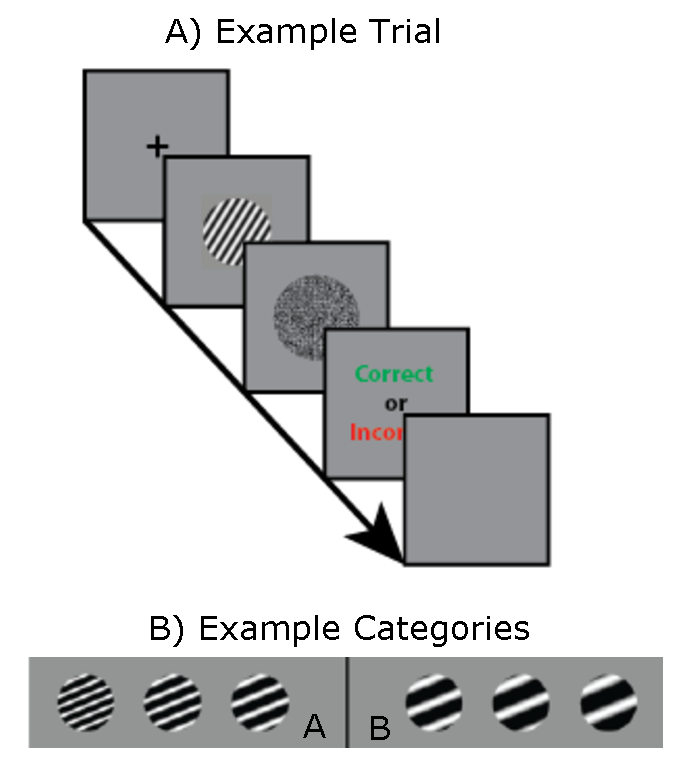
\includegraphics[width=.35\textwidth]{figures/Cats.pdf}
  \caption{Example trial and category problem. A) Events that occurred on each
    trial. B) An example of a typical category structure.}
  \label{trial}
\end{figure}

Participants were explicitly told the relevant dimension, as well as the generic
response mapping (e.g., thick bars = `A', thin bars = `B'). Figure \ref{trial}
shows the structure of an example trial, along with an example of a typical
category structure. All trials in every condition included a 500 ms fixation
cross, a response-terminated stimulus, a circular white-noise mask, corrective
feedback, and an inter-trial interval (ITI) that varied according to condition.
The text `Correct' was displayed in centered, large green font after correct
responses, and the text `Incorrect' was displayed in centered, large red font
after incorrect responses.

The three conditions are described in Table \ref{conditions}. In the Delay
condition, feedback was delayed 3.5 s after the response and the ITI was 0.5 s.
There were two immediate feedback control conditions in which feedback was given
0.5 s after the response. The Short ITI had the same ITI as the Delay condition
and the Long ITI had the same trial duration as the Delay condition (i.e., the
same inter-stimulus interval).

\begin{table}
    \caption{Durations (in s) of Trial Events in each Condition}
    \label{conditions}
    \begin{tabular}{c|cccc}
      Conditions & Stim & Mask & FB & ITI \\[0.5ex]
      \hline\\[-1.5ex]
      Delay & RT & 3.5 & 1.0 & 0.5 \\[0.5ex]
      \hline
      Immediate/Short ITI & RT & 0.5 & 1.0 & 0.5 \\[0.5ex]
      \hline
      Immediate/Long ITI & RT & 0.5 & 1.0 & 3.5 \\[0.5ex]
    \end{tabular}
\end{table}

\section{Results}
INSERT FINAL PROJECT RESULTS HERE.

\bibliography{sample}

\section{Author Notes}
Preparation of this article was supported by Public Health Service Grant
MH2R01-063760.

\end{document}